\documentclass[../rapport_MVEX01-11-05]{subfiles}
\begin{document}
De metoder som använts ger en träffsäkerhet på 91.4\,\% för de tio statiska
gesterna. Denna träffsäkerhet kan sannolikt förbättras på ett antal
olika sätt, dessutom
kan metoden utökas och generaliseras för att kunna identifiera
dynamiska gester. I detta kapitel presenteras förslag på möjliga framtida
förbättringar och utökningar av metoden samt exmepel på tillämpningar.

\section{Hudigenkänning}
De sannolikhetsfördelningar som används för att skilja hud från annat
fungerar tillräckligt bra för att kunna skilja ut handen i en
relativt kontrollerad miljö, men bättre resultat skulle kunna uppnås
med bättre sannolikhetsfördelningar. En sak man skulle kunna göra
är att använda Gaussian Mixture Models, d.v.s.~linjärkombinationer av flera
sannolikhetsfördelningar, inte bara för hud utan även för ickehud.
Detta bidrar till att problematiska färger, som ofta klassas fel,
kan ''filtreras bort''.
Bättre fördelningar skulle
antagligen även fås med en större datamängd, alltså fler
exempelbilder.

Man kan också använda någon annan klassificerare, såsom \knn,
vid skapandet av hudfärgskartan. Ett problem med den metoden är att det
kräver att man kasserar data för att få lika stora prototypmängder,
eller att man viktar datapunkterna.
Efter det statistiska urvalet skulle man kunna redigera direkt i
hudfärgskartan för att få ett bättre resultat.

En robustare metod är eventuellt den adaptiva metod som föreslås av
\citeasnoun{Hassanpour08}, där klassificerade sammanhängade
hudområden återkopplas till beräkningen av fördelningarna.
På så vis anpassas kontinuerligt hudfärgsfördelningarna till miljön.
Slutligen kan en mer omfattande filtrering och bildbehandling användas
för att fylla i de ''hål'' som bildas i handen (se figur
\vref{fig:hudklassificering}).

\section{Handidentifiering}
Handidentifieringen kan förbättras på ett antal punkter;
den metod vi använder, att söka ett tillräckligt stort objekt från höger i
bilden, är relativt ''dum''. Förutsätter man att de två objekt som kan finnas
i bilden är ett ansikte och en hand (vilket ofta är fallet) så kan man
istället välja handen genom att först identifiera ansiktet, exempelvis genom
den metod \citeasnoun{Hsu02} använder, för att sedan ''välja bort'' detta
objekt (dvs.~ta bort det från bilden). Vad som då finns kvar i bilden bör vara
handen (om brus först tagits bort eller om de två största
objekten i bilden redan isolerats enligt \citeasnoun{Nielsen04}).

Man kan dessutom klippa bort handleden på det sätt
\citeasnoun{Deimel99} föreslår, och därmed öka träffsäkerheten --- att
handleden ibland syns och ibland skuggas är något som gör vissa av 
egenskaperna alltför osäkra. Dessutom skulle man då kunna släppa på kravet
att användaren bär en långärmad tröja.

Till sist kan man då handen identifierats utnyttja
vetskapen om dess läge, och
klippa bort resten av bilden i nästa bildruta.
På så vis minskar risken för att man tappar bort handen och
klassar ett annat objekt som handen.

\section{Egenskaper}
De egenskaper som använts för klassificering av gesterna har visat sig relativt
effektiva, men det finns modifieringar och tillägg som skulle kunna
öka träffsäkerheten. 

En sådan modifiering är att istället för fyrkantigheten $\Delta
x/\Delta y$ använda dess logaritm, $\ln(\Delta x/\Delta
y)$, eftersom kvotens värdemängd är $(0,\infty)$ och tar värdet 1 då
höjen och bredden är samma, vilket innebär att egenskapen får större
viktning då handens utsträckning är horisontell än när den är vertikal. Detta problem
försvinner när kvoten logaritmeras. Även övriga egenskaper som
definieras genom kvoter kan logaritmeras på samma sätt.

Det finns också hela klasser av egenskaper som inte använts.
Genom studier av handens kurvatur kan fingertoppar 
identifieras --- antal, avstånd och relativt läge för dessa är
mycket intressanta egenskaper, och ger antagligen ett bra resultat.
En annan intressant egenskapsklass är de som utnyttjar mönster i det
inre av handen, tidigare analyserades enbart egenskaper för den binära bilden.
Detta skulle kunna göras
genom att man efter att ha identifierat handen studerar den
i originalbilden, t.ex.~genom ett kantdetektionsfilter.
I den resulterande ''kantbilden'' kan sedan riktningar och antal kanter
beräknas med hjälp av en så kallad Houghtransform \cite{Duda72}.

\subsection{Val av egenskaper}
Att klassificeringsresultaten från framåturval och bakåteliminering är 
identiska, trots skillnaden i antal egenskaper, gör att andra
optimeringsrutiner är värda att undersöka.
Ett mer sofistikerat prototypurval och ''cross validation'' är exempel
på förbättringar.

\section{\knn}
För att förbättra \knn-metodens träffsäkerhet kan först och
främst prototypmängden utökas till fler punkter per gest. En annan
möjlighet är att inspektera de bilder som faktiskt ligger bakom
punkten i egenskapsrummet. Om en bild är uppenbart felaktig, och kanske hade varit
svår att tolka som rätt gest även för en människa, kan den med fördel tas bort.
Slarvigt utförda gester kommer då mindre sannolikt att
klassificeras rätt.

Man kan även införa ett tröskelvärde på avståndet till de närmsta
prototypobjekten, över vilket gesten inte klassificerades som någon
gest. På detta sätt kan man löpande söka efter gester
i en filmsekvens, ett viktigt steg mot
realtidsidentifiering.

Det största problemet med den metod som beskrivs i rapporten är dock
inte implementationen utan testandet av den. Då vi tagit fyra
efterföljande bilder
från varje film i testmängden är datan inte oberoende. Tvärtom är det
mycket troligt att samtliga fyra bilder ska klassas likadant, varför
den effektiva testmängden inte är mycket mer än 16 bilder per
gest. Denna mängd är egentligen för liten för att kunna dra några
säkra slutsatser om klassificerarens prestanda.

\section{Realtid}
Målet med en applikation för gestigenkänning är givetvis att kunna tolka
gester i realtid, vilket kan vara svårt eftersom bildbehandlingen och
klassificeringen som används ofta är beräkningsintensiv. Vår implementering
är skriven i \MATLAB, och skulle bli mycket snabbare om den
skrivs i ett lågnivåspråk som C istället, men kan trots det utföra
beräkningarna snabbt nog för att nästan vara realtid.
Ju fler egenskaper man lägger till och mer förfinad analys, desto
större blir naturligtvis beräkningskraven. Detta är framförallt
viktigt vid tillämpningar i robotar och inbyggda system, där beräkningskraften
är begränsad.

För att kunna känna igen statiska gester behövs betydligt färre bilder per
sekund än de 24 webbkameran ger. Därmed kan man nöja sig med
att behandla fyra eller sex bilder per
sekund, vilket gör att gestigenkänningen ser ut att vara i realtid.
Detta medför givetvis att statiska gester som visas i mindre tid
än intervallet mellan bilderna inte skulle kännas igen.

\section{Tillämpningar}

\notes{Skriv eller ta bort}
sluta med avancerade emotionella robotar typ..

\section{Dynamiska gester}
För att på allvar uppnå den potential människa-dator-interaktion för med sig
är det viktigt att även kunna klassificera dynamiska gester.
Med den HMM-metod vi utformat befinner vi oss på gränsen till
att nå resultat och att kunna avgöra hur väl den fungerar i praktiken.

Eftersom metoden behandlar dynamiska gester som flera 
statiska i följd återkommer flera av utmaningarna förknippade med dessa. 
Beräkningsintensiteten tilltar i och med implementeringen av HMM, vilket innebär 
att \MATLAB antagligen blir otillräckligt.

Eftersom en dynamisk gest består av flera statiska
kommer också skillnaden mellan likadana dynamiska gester att öka. Detta leder till 
mer jobb under träningsfasen, då fler filmsekvenser kan behövas för att få en 
bra prototypmängd, och för att träna HMM:er till att klara av variationerna. 
Man måste även introducera nya egenskaper som karakteriserar dynamiska gester, 
exempelvis position och hastighet.

I ett tidigt skede bearbetade vi även dynamiska gester.
I figur \vref{fig:motion} visas hur egenskaperna då ser ut.
Dessa tidsberoende egenskaper kan analyseras exempelvis
med hjälp av waveletanalys \cite{Hastie09}. 

\begin{figure}[tbp]
    \begin{center}
        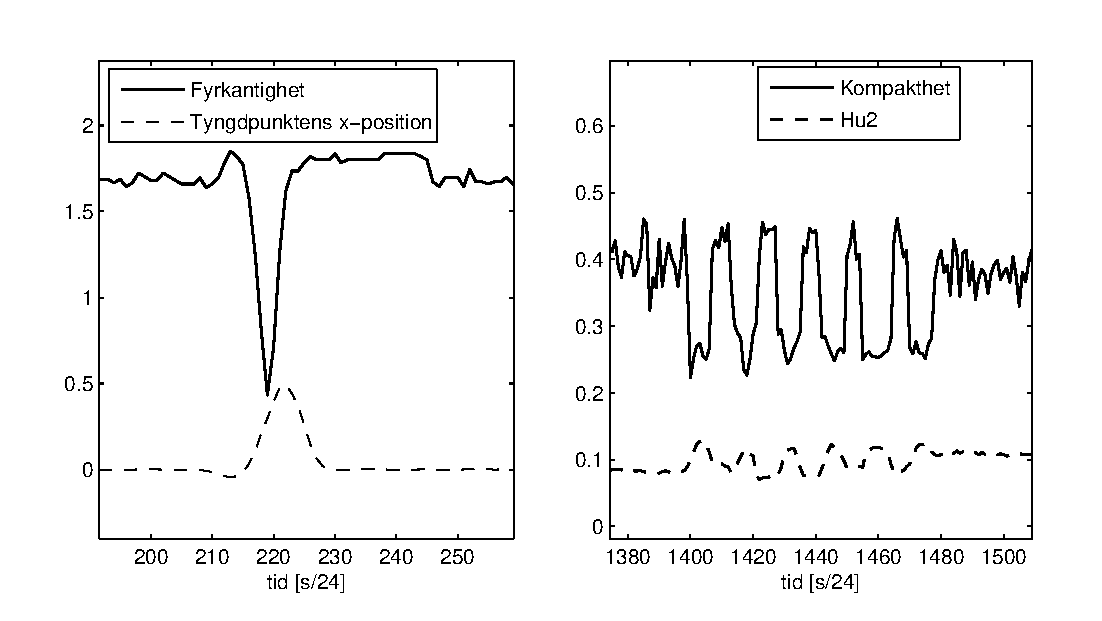
\includegraphics[width=\columnwidth]{bilder/motion}
    \end{center}
    \caption{BILD}
    \label{fig:motion}
\end{figure}

\section{Slutsats}
Med det ramverk för analys som presenterats, och med koden i bilaga
\ref{sec:matlab} som utgångspunkt kan dessa förslag relativt enkelt
implementeras och testas.

\notes{skriv nåt käckt här?}
\end{document}
